\documentclass{article}
\usepackage{amsthm, amsmath, amssymb}
\usepackage{graphicx}
\usepackage{rotating}

\newtheorem{claim}{Claim}
\newtheorem{theorem}{Theorem}
\newtheorem{define}{Definition}

\newcommand{\R}{\mathbb{R}}
\newcommand{\relint}{\mbox{\textup{relint}}}
\newcommand{\trp}{\mbox{${}^{\top}$}}
\newcommand{\trace}{\mbox{tr}}
\newcommand{\argmin}{\mbox{\textup{argmin}}}
\newcommand{\N}{\mathcal{N}}

\title{Fundamentals of Bregman Divergences}

\begin{document}
\maketitle

\section{Introduction}
Bregman divergences were introduced by Bregman in \cite{b.67} and have
traditionally been studied by researchers in the optimization and
numerical analysis communities.  The book \cite{cz.97} contains a
detailed overview of Bregman divergences and their application in
iterative optimization algorithms.  Within machine learning, Bregman
divergences first appear in work on iterative scaling \cite{ldd.97}
and online learning, \textit{e.g.} 
\cite{gls.97,hw.98,aw.01} and were later identified with the $k$-means
algorithm \cite{bm.05}.   

\section{Definition and Motivation}
In this section we explain what a bregman divergence is and why they
are compelling objects of study.  These divergences arise naturally
from a surprisingly disparate collection of sources.  We consider
four.  First, they are a key ingredient in iterative optimization
schemes for convex optimization.  Second, they have a deep connection
to the exponential family of probability distributions.  Third, they
arise out of basic axioms in connection with maximum likelihood
estimation.  Finally, they satisfy certain mathematical properties
that make them a central concept in information geometry.  
%Their basic
%mathematical properties show them to be a generalization of $\ell_2^2$
%and the relative entropy, connecting them to the $k$-means algorithm.  

\subsection{Formal Definition}
\begin{define}
Let $f:C \subset \R^D \rightarrow \R$ be a strictly convex function that is
differentiable on the relative interior of $C$.  The bregman divergence based
on $f$ is defined as
\begin{align*}
  d_f(x,y) \equiv f(x) - f(y) - \langle \nabla f(y),x-y \rangle.  
\end{align*}
Note that $d_f:C \times \relint(C) \longrightarrow \R_+$.  
\end{define}
A bregman divergence measures the distance between $f$ and its
first-order taylor expansion.  See figure \ref{fig:bregDef}.  Table
\ref{tbl:bregdivs} lists some common bregman divergences.  


\begin{figure}
\begin{center}
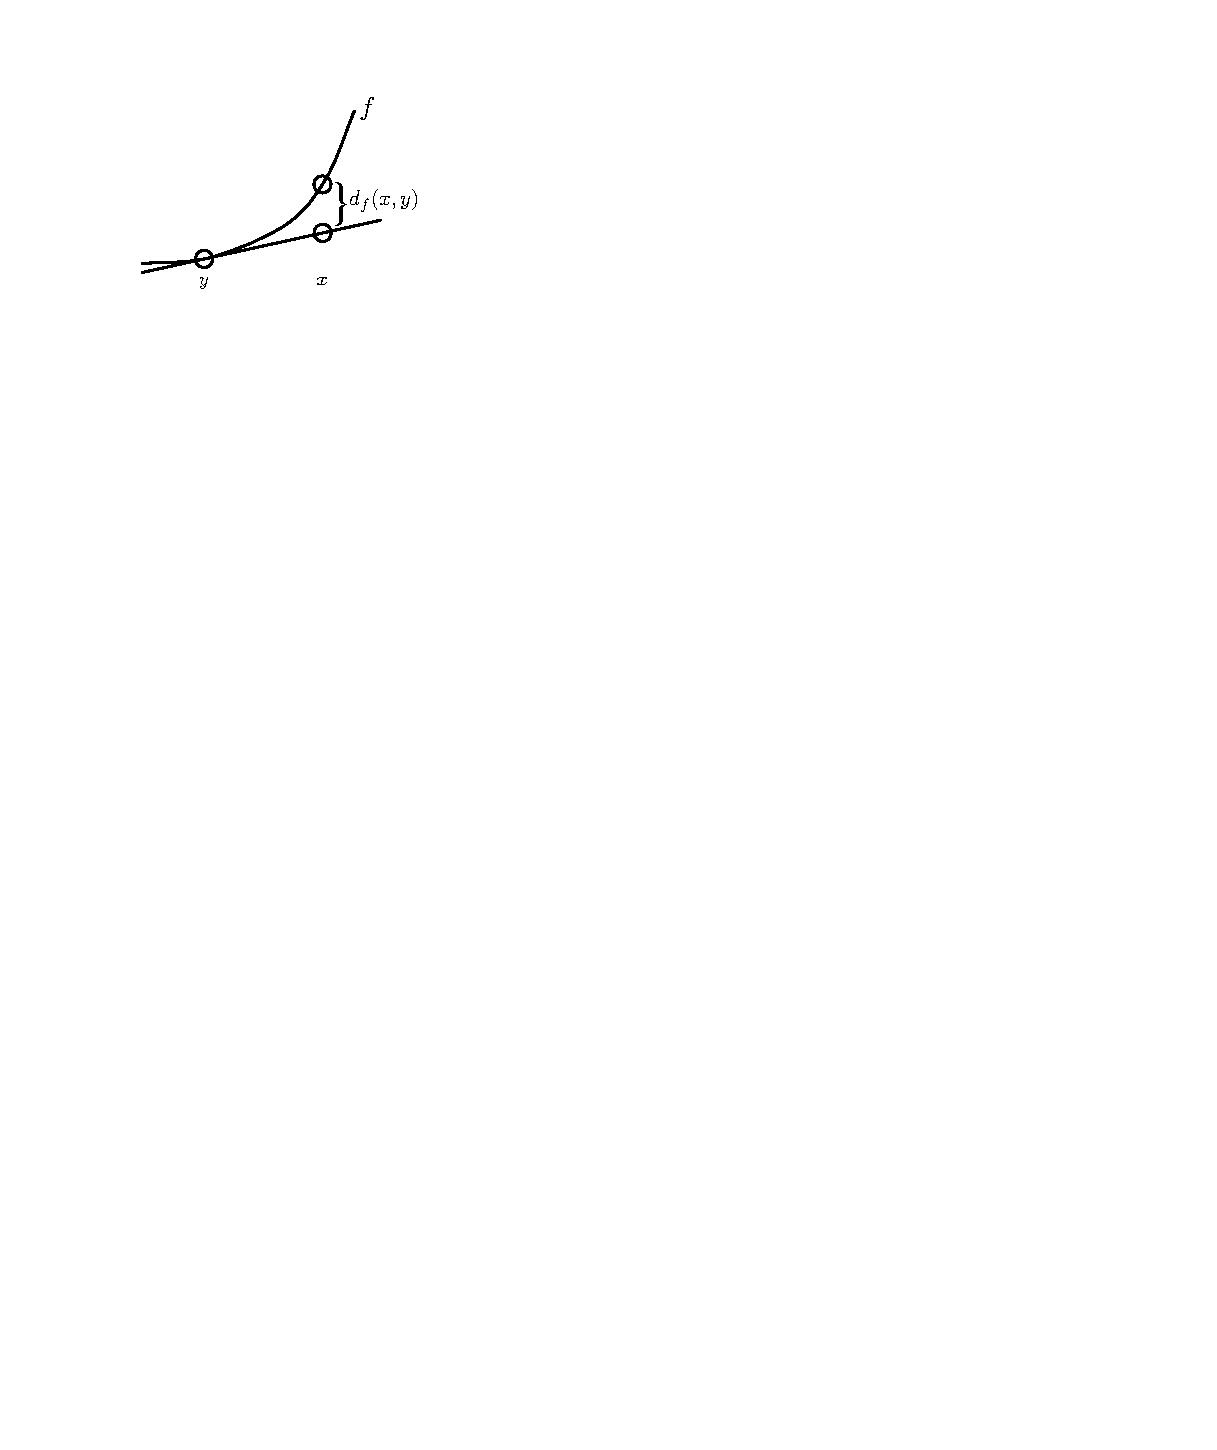
\includegraphics[width=0.35\linewidth, height=!]{figs/bregDef.pdf}
\caption{The bregman divergence between $x$ and $y$.}
\label{fig:bregDef}
\end{center}
\end{figure}

\begin{sidewaystable}
\renewcommand\arraystretch{1.75}
\begin{center}
\caption[Standard bregman divergences.]{Standard bregman divergences.
  $S_{++}^D$ denotes the cone of positive definite $D\times D$ matrices.}  \label{tbl:bregdivs}
\vspace{.5cm}
\begin{tabular}{c|c|c|c}
\textbf{Name} & \textbf{Domain} & \textbf{Base function} &$d_f(x,y)$ \\\hline
$\ell_2^2$ & $\R^D$ & $\frac{1}{2}\|x\|_2^2$ & $\frac{1}{2}\|x-y\|^2_2$\\
Mahalanobis ($Q \succ 0$) &$\R^D$ & $\frac{1}{2}x\trp Q x$ &$\frac{1}{2}(x-y)\trp Q (x-y)$\\
KL-Divergence & $\R^D_+$& $\sum x_i \log{x_i}$ & $\sum
x_i\log{\frac{x_i}{y_i}} - x_i + y_i$ \\
Itakura-Saito & $\R^D_+$ &  $-\sum\log{x_i}$ &
$\sum\left(\frac{x_i}{y_i} - \log{\frac{x_i}{y_i}} -1\right)$\\
Exponential & $\R^D$ & $\sum e^{x_i}$ & $\sum
e^{x_i}-(x_i-y_i+1)e^{y_i}$\\
Bit Entropy & $[0,1]^D$ & $\sum(x_i\log{x_i}+(1-x_i)\log{(1-x_i)})$ &
$\sum(x_i\log\frac{x_i}{y_i}+(1-x_i)\log(\frac{1-x_i}{1-y_i}))$ \\
Hellinger & $[-1,1]^D$ & $-\sum{\sqrt{1-x_i^2}}$ & 
$\sum\frac{1-x_iy_i}{\sqrt{1-y_i^2}} - \sqrt{1-x_i^2}$ \\
$\ell_p^p$, $p\in [1,\infty]$ & $\R^D$ & $\|x\|_p^p$ & $\sum |x_i|^p
-px_i\mbox{sgn}(y_i)|y_i|^{p-1}+(p-1)|y_i|^p$\\
Log-det & $S^D_{++}$ & $-\log\det{X}$ & $\langle X,Y^{-1} \rangle
-\log\det{XY^{-1}} -N$ \\
von Neumann entropy & $S_{++}^D$ & $\trace\left(X \log{X}-X\right)$ &  $\trace\left(X(\log{X}-\log{Y})-X+Y\right)$
\end{tabular}
\end{center}
\renewcommand\arraystretch{1}
\end{sidewaystable}

It is often assumed that $f$ is not only strictly convex but is also
\emph{Legendre}.  A function $f:C\rightarrow \R$ is Legendre if 
\begin{itemize}
\item $C \neq \emptyset$ and its interior is convex;
\item $f$ is strictly convex and has continuous first partial
  derivatives; and
\item if $x_1,x_2,\ldots \in C$ is a sequence converging to a boundary
  point of $C$, $\|\nabla f(x_n) \| \rightarrow \infty$.
\end{itemize}
These additional requirements aid in the analysis of certain iterative
projection algorithms \cite{cz.97}.  

The strict convexity of $f$ implies that a bregman divergence is
always non-negative and equal to zero only if its two arguments are
identical.  It is similarly easy to check that a bregman divergences
is convex in its first argument, but not necessarily in its second.  

\subsection{Convex optimizaton}

\subsection{Exponential families}
There is a remarkable connection between bregman divergences and
exponential families.  We sketch the basic details in this
section.  

Let $\nu$ be a $\sigma$-finite measure defined on the Borel subsets of
$\R^D$.  An  exponential family
consists of all distributions with probability density functions of the form
\begin{align*}
p_{\eta}(x) = \exp(\langle\eta,T(x) \rangle - G(\eta))\;\nu(x),
\end{align*}
where $T(x)$ is a sufficient statistic.  We focus on the case where
$T(x)=x$; these are called \emph{regular} exponential families.  
The set of all $\eta$ such that 
\begin{align*}
\int e^{\langle \eta,x \rangle} \nu(dx) < \infty
\end{align*}
is called the \emph{natural parameter space}.  The function $G(\cdot)$ normalizes
the probability distribution and is called the \emph{log partition
function}.  It is equal to
\begin{align*}
G(\eta) = \log \int e^{\langle \eta,x \rangle } \nu(dx).
\end{align*}

Many standard distributions are examples of regular exponential
families.  One example is the Bernoulli distribution, with
pdf 
\begin{align*}
p(x) = \left\{\begin{array}{cc} \mu & \mbox{for }x=1\\
1-\mu & \mbox{for } x=0
\end{array} \right. = \mu^x(1-\mu)^{1-x}.
\end{align*}
Let $\eta = \log\frac{\mu}{1-\mu}$.  Then 
\begin{align*}
p(x) = \exp(x\cdot\eta - \log(1+e^{\eta})),
\end{align*}
so is an exponential family with log partition function
$\log(1+e^{\eta})$.  Notice that the natural parameter space is all of
$\R$, whereas the expectation $\mu$ is confined to $[0,1]$.  

Another example is the univariate Gaussian distribution
$\N(\mu,\sigma^2)$, with pdf 
\begin{align*}
p(\omega) = \frac{1}{\sqrt{2\pi}\sigma}e^{-(\omega-\mu)^2/2\sigma^2}.
\end{align*} 
Re-parametrizing with $x\equiv (\omega,\omega^2)$ and $\eta \equiv
(\frac{\mu}{\sigma^2},-\frac{1}{2\sigma^2})$ puts $p(x)$ into standard
exponential form.  

A third example is the Poisson distribution, with pdf 
\begin{align*}
p(x) = \frac{\lambda^xe^{-\lambda}}{x!},
\end{align*}
which is defined over $\N$ for $\lambda\in\R_+$.  Setting $\nu(x) =
\frac{1}{x!}$ and $\eta = \log(\lambda)$ recovers the familiar
exponential form.  
 
There are many other examples, including the binomial and exponential
distributions, multidimensional Gaussian distribution, and the
multinomial distribution.  

The log-partition function has many useful properties. Here we need
only a couple of essential ones.  First, the gradient of $G(\eta)$
is the mean of the corresponding exponential distribution:
\begin{align*}
\nabla G(\eta) = \int x p_\eta(x) \nu(dx).
\end{align*}
Additionally, the Hessian of $G(\eta)$ is equal to covariance matrix of
$p_\eta$.  Because the gradient is equal to the mean, the gradient can be
thought of as providing a link between the natural parameter space and
the expectation parameter space.  Another fact of the log-partition
function is that it is strictly convex (assuming ${p_\eta}$ is
minimal), and in fact is Legendre \cite{bm.05}.  Thus the convex
conjugate is defined, and $\nabla G^*(y)$ provides the inverse mapping
from the space of expectation parameters to the space of natural
parameters.  

Suppose we wish to measure how similar two members of an exponential
family are.  A natural way to do this is to compute the KL-divergence
between them, and this is where the connection to bregman divergences
becomes apparent.  Let $p(x)$ and $q(x)$ be members of an exponential
family with natural parameters $\eta_1$ and $\eta_2$ respectively.
Then the KL-divergence between them is
\begin{align*}
\int p(x) \log\frac{p(x)}{q(x)}dx &=\int p(x)\log\frac{\exp(\langle\eta_1,x\rangle
  -G(\eta_1))}{\exp(\langle\eta_2,x\rangle -G(\eta_2))} dx\\
&= \int p(x) (\langle \eta_1-\eta_2,x\rangle +G(\eta_2) - G(\eta_1)
)dx\\
&= \langle \nabla G(\eta_1), \eta_1-\eta_2 \rangle + G(\eta_2) -
G(\eta_1), \quad\mbox{since }\nabla G(\eta)\mbox{ is the mean} \\
&=d_G(\eta_2,\eta_1).
\end{align*}
Thus the entropy between two members of an exponential family is the
bregman divergence based on the log-partition function between their
natural parameters.  Moreover, we can write the pdf of any regular
exponential family in terms of a bregman divergence:
\begin{align*}
p_{\eta}(x) &= \exp(\langle x,\eta \rangle - G(\eta)) \nu(x)\\
&= \exp(G^*(\eta ')+ \langle x-\eta',\eta \rangle - G^*(x)+G^*(x))
\nu(x)\\
&=\exp(-d_{G^*}(x,\eta') + G^*(x) )\nu(x).
\end{align*}
Since $\eta'$ is the mean of $p_{\eta}$, this equality shows
that the pdf is a function of the divergence between $x$ and the mean.
Similarly, 
\begin{align*}
p_{\eta}(x) = \exp(-d_G(\eta,x') + G^*(x))\nu(x),
\end{align*}
where $x'\equiv \nabla G^*(x)$.  

The connection between bregman divergences and exponential families
goes a bit deeper.  Here, we showed that for exponential family, there
is a related bregman divergence.  In \cite{bm.05}, it is shown that
there is a one-to-one correspondence between the regular exponential
families and the so-called regular bregman divergences---bregman
divergences defined over a restricted class of convex base functions.  

\section{Geometry}
\subsection{Pythagorean theorem}
The pythagorean theorem is a key property of bregman divergences that
governs the geometry of bregman projections.  This theorem 
underlies some of the bregman geometry we develop in chapter
\ref{chap:bbtree}, even though it is not explicitly used.  
\begin{theorem} Let $C$ be a closed convex set and let $y = \argmin_{y \in C}
  d_f(y,z)$ be the bregman projection of $z$ onto $C$.  Further suppose
  that $x\in C$.  Then 
\begin{align*}
d_f(x,z) \geq d_f(x,y) + d_f(y,z).
\end{align*} \label{thm:pythagineq}
\end{theorem} 
\begin{proof}
Define $G(x) = d_f(x,y)-d_f(x,z)$.  Then
\begin{align*}
G(x) &= f(x)-f(y) - \langle \nabla f(y),x-y\rangle - \left(
  f(x)-f(z)-\langle \nabla f(z),x-z \rangle \right)\\
&= f(z) + \langle \nabla f(z),x-z \rangle - f(y) - \langle \nabla
f(y), x-y \rangle,
\end{align*}
so $G$ is linear in $x$.  Moreover $G(y)= d_f(y,y) - d_f(y,z) =
-d_f(y,z)$. Let $\alpha \in [0,1]$ and $x_\alpha = \alpha x + (1-\alpha)y$.   
\begin{align*}
G(x_\alpha) = G(\alpha x + (1-\alpha) y) &= \alpha G(x) +
(1-\alpha)G(y) \\
&= \alpha (d_f(x,y)-d_f(x,z) +d_f(y,z)) -d_f(y,z).
\end{align*}
Also,
\begin{align*}
G(x_\alpha) =d_f(x_\alpha,y) - d_f(x_\alpha,z),
\end{align*}
so, when $\alpha>0$,
\begin{align*}
d_f(x,y) +d_f(y,z) - d_f(x,z) = \frac{d_f(y,z)+ d_f(x_\alpha,y) -
  d_f(x_\alpha,z)}{\alpha}.
\end{align*}
We show that the right hand side is less than or equal to zero.  Since
$x_\alpha \in C$ and $y$ is the projection of $z$ onto $C$, $d_f(y,z)
\leq d_f(x_\alpha,z)$. Thus we only need to show that
$\frac{d_f(x_\alpha,y)}{\alpha} \leq 0$ for some $\alpha$.  We do this
by taking the limit as $\alpha\rightarrow 0$ from the right:  
\begin{align*}
\lim_{\alpha\rightarrow 0} \frac{d_f(x_\alpha,y)}{\alpha} &=
\lim_{\alpha\rightarrow 0} \frac{f(\alpha x+ (1-\alpha)y) - f(y)
  -\langle \nabla f(y),\alpha x-\alpha y\rangle}{\alpha} \\
&= \lim_{\alpha\rightarrow 0} \frac{f(\alpha x + (1-\alpha)y) -
  f(y)}{\alpha} - \lim_{\alpha\rightarrow 0} \frac{\langle \nabla
  f(y),\alpha x + (1-\alpha)y -y \rangle}{\alpha}\\
&= \langle \nabla f(y),x-y \rangle - \lim_{\alpha\rightarrow 0}
\langle \nabla f(y),x-y \rangle \quad \mbox{ (by
  l'H\^{o}pitals rule) } \\
&= 0. 
\end{align*}
\end{proof}
The previous inequality becomes an equality if $C$ is an affine space.
\begin{theorem} Let $C$ be an affine space and let $y=\argmin_{y\in C}
  d_f(y,z)$ be the bregman projection of $z$ onto $C$.  Let $x\in C$.
  Then
\begin{align*}
d_f(x,z) = d_f(x,y) + d_f(y,z).
\end{align*}
\end{theorem}
\begin{proof}
Let $x'$ be any point in $C$, and set $\lambda$ to satisfy 
$y=\lambda x+ (1-\lambda) x'$.  
Define $x_\alpha = \alpha x + (1-\alpha)
x'$, and let $G(x) = d_f(x,y) - d_f(x,z)$.  Since $G(x_\alpha) =
d_f(x_\alpha,y) - d_f(x_\alpha,z)$,
\begin{align}
\frac{\partial G(x_\alpha)}{\partial \alpha} =
\frac{\partial}{\partial \alpha} d_f(x_\alpha,y) -
\frac{\partial}{\partial \alpha} d_f(x_\alpha,z). \label{eq:derivs}
\end{align}
Note that $x_{\alpha}\in C$; since $y$ is the projection of $z$ onto
$C$ and $x_\alpha = y$ when $\alpha=\lambda$, $d_f(x_\alpha,z)$ is
minimized at $\alpha=\lambda$.  Moreover, $d_f(x_\alpha,y)$ is also
minimized at $\alpha=\lambda$ (it is zero there).  Thus, both 
divergences on the right of (\ref{eq:derivs}) are minimized at
$\alpha=\lambda$, implying $\left. \frac{\partial
  G(x_\alpha)}{\partial \alpha} \right|_{\alpha = \lambda} = 0$.

Using the linearity of $G$ (see the proof of theorem
\ref{thm:pythagineq}), we can expand 
\begin{align*} 
G(x_\alpha) &= d_f(x_\alpha,y) - d_f(x_\alpha,z) \\
&= \alpha (d_f(x,y) - d_f(x,z)) + (1-\alpha) (d_f(x',y) - d_f(x',z)).
\end{align*}

Differentiating with respect to $\alpha$, we get
\begin{align*}
\frac{\partial G(x_\alpha)}{\partial \alpha} = d_f(x,y)-d_f(x,z) - d_f(x',y)
+ d_f(x',z).
\end{align*}
At $\alpha=\lambda$, $\frac{\partial G(x_\alpha)}{\partial \alpha}=0$,
so
\begin{align*}
d_f(x,y)-d_f(x,z) - d_f(x',y)
+ d_f(x',z)=0.
\end{align*}
This equality is true for all $x' \in C$, so picking $x'=y$, we get 
\begin{align*}
d_f(x,z) = d_f(x,y) + d_f(y,z).
\end{align*}
\end{proof}

\subsection{Conjugacy} \label{sec:conjugate}
Conjugacy is a central duality notion used in convex analysis \cite{r.70}.
\begin{define}
The \emph{convex conjugate} of a function $f: \R^d\rightarrow \R$ is
\begin{align*}
f^*(x) = \sup_y \left\{\langle x,y \rangle - f(y) \right\}.
\end{align*}
\end{define}
The definition of a conjugate function immediately yields the 
\emph{Fenchel-Young inequality}:
\begin{align*}
f(x) + f^*(y) \geq \langle x,y \rangle.
\end{align*}
If $f$ is differentiable, we can compute $f^*$ by setting the
derivative to zero:
\begin{align*}
&\nabla_y \left( \langle x,y \rangle - f(y) \right)  = x - \nabla f(y)
= 0\\
&\Longrightarrow x = \nabla f(y)\\
&\Longrightarrow y = (\nabla f)^{-1}(x).
\end{align*}
Thus
\begin{align}
f^*(x) = \langle x, (\nabla f)^{-1}(x) \rangle - f( (\nabla
f)^{-1}(x)). \label{eq:conjdef}
\end{align}
A crucial property of the conjugate function is that its gradient
is an inverse to the gradient of the original function.  To keep
notation clean, define $h(x) \equiv \nabla f(x)$.  Then, following the
above derivation, we have
\begin{align*}
f^*(x) &= \langle x,h^{-1}(x) \rangle - f(h^{-1}(x)); \mbox{ implying
  that }\\
\nabla f^*(x) &= h^{-1}(x) + \nabla h^{-1}(x) \cdot x - \nabla
h^{-1}(x) \nabla f(h^{-1}(x))\\
&=h^{-1}(x)\mbox{\;\; (since }\nabla f(x) = h(x)).  
\end{align*}
Thus $\nabla f$ and $\nabla f^*$ are inverses of one-another.  

Let $x' \equiv \nabla f(x)$ and $y' \equiv \nabla f(y)$.  
Then plugging $x'$ and $y'$ into (\ref{eq:conjdef}), we get the
convenient relations 
\begin{align*}
f^*(x') &= \langle x',x \rangle - f(x) \quad \mbox{and}\\
f^*(y') &= \langle y',y \rangle - f(y).
\end{align*}
Let us now consider the bregman divergence 
associated with $f$ in light of the conjugate function. We show
that $d_{f^*}(y',x') = 
d_f(x,y)$. 
\begin{align*}
d_{f^*}(y',x') &= f^*(y') - f^*(x') - \langle \nabla f^*(x'), y'-x'
\rangle \\
&= \langle y',y \rangle -f(y) - \langle x,x' \rangle + f(x) - \langle
\nabla f^*(x'), y'-x' \rangle\\
&= f(x) - f(y) -\langle x',x \rangle + \langle y',y
\rangle - \langle x,y' - x' \rangle \quad
\mbox{(since $x = \nabla f^*(x')$)}\\
&= f(x) - f(y) - \langle \nabla f(y),x-y \rangle \\
&= d_f(x,y).
\end{align*}
This equality is useful because it permits algorithms designed to
optimize over the first argument to work over the second argument.  It
provides an elegant way to sidestep the asymmetry of bregman
divergences.  See section \ref{sec:rnn} for an example.

Another easily derived equality is 
\begin{align} 
d_f(x,y) = f(x) + f^*(y') - \langle x,y'\rangle . \label{eq:breg-youngs}
\end{align}
This equality reveals another interpretation interpretation of a
bregman divergence: it is a measurement of the slackness in the
Fenchel-Young inequality. 

\subsection{Centroidal property}
Bregman divergences satisfy a centroidal property that makes them
amenable to $k$-means style clustering \cite{bm.05}.  This property states
that the average divergence from a point to a set can be decomposed as
the divergence from the point to the set's centroid plus the average
divergence from the set to the centroid.  
\begin{theorem}
Let $S \subset \R^d$ be a set of size $n$ and let $d_f(S,x)$ denote
$\sum_{s\in S} d_f(s,x)$.  Let $\mu = \frac{1}{n}\sum_{s\in S} s$ be the mean of
$S$.  Then for all $x \in \R^d$, 
\begin{align*}
d_f(S,x) = d_f(S,\mu) + n d_f(\mu,x).
\end{align*}
\end{theorem}
\begin{proof}
Expanding the right side, we have
\begin{align*}
d_f&(S,\mu) + n \cdot d_f(\mu,x) \\
&= \sum_s f(s) - n f(\mu) - \sum_s \langle \nabla
f(\mu),s-\mu \rangle +n f(\mu) - n f(x) - n \langle \nabla f(x),\mu-x \rangle\\
&= \sum_s \left( f(s) - f(x) \right) - \sum_s \langle \nabla
f(\mu),s-\mu \rangle - n \langle \nabla f(x),\mu-x \rangle \\
&= \sum_s \left( f(s) - f(x) \right) - \left\langle \nabla f(\mu),\sum_s s-
n \mu \right\rangle - \langle \nabla f(x),n\mu-nx \rangle \\
&= \sum_s \left( f(s) - f(x) \right) - \left\langle \nabla f(x),\sum_s
(s-x) \right\rangle \\
&= \sum_s \left( f(s) - f(x) - \langle \nabla f(x),s-x \rangle \right)
\\
&= d_f(S,x).
\end{align*}
\end{proof}


\subsection{Other technical results}
One convenient property of bregman divergences is that they can by
composed.  Suppose that $\{f_i\}$ are strictly convex functions and
$\{\alpha_i\}$ is a set of non-negative numbers.  Then $g\equiv\sum\alpha_i
f_i$ is also a strictly convex function. Thus we can define a bregman
divergence based on $g$
\begin{align*}
d_g(x,y) &= \sum \alpha_i f_i(x) - \sum\alpha_i f_i(y) -\langle \nabla
\left[ \sum\alpha_i f_i(y)\right],x-y \rangle\\
&= \sum \alpha_id_{f_i}(x,y).
\end{align*}
Similarly, one can define a $D$-dimensional multivariate bregman
by summing $D$ one-dimensional bregman divergences coordinate-wise.
These properties are useful for working with mixed-type data.  For
example, a point $x$ might have a histogram component of, say, the first
10 coordinates, and a vector coordinate of the next 5 coordinates.
A reasonable way to compute the distance between two such points would
be to measure the KL-divergence between the first 10 coordinates, and
the $\ell_2^2$ distance between the last 5.  Any machinery defined for
arbitrary bregman divergences, such as the fast NN algorithms
developed in this dissertation, will be able to handle this mixed-type
divergence as it is itself a bregman divergence.  


In the proof of theorem \ref{thm:pythagineq}, we showed that the
difference $G(x)=d_f(x,y) - d_f(x,z)$ is linear in $x$:
\begin{align*}
G(x) &= f(x)-f(y)- \langle \nabla f(y),x-y \rangle -\left( f(x) - f(z)
  -\langle f(z),x-z \rangle \right)\\
&= f(z) + \langle \nabla f(z),x-z \rangle - f(y) - \langle \nabla
f(y), x-y \rangle.
\end{align*}
In particular, this means that the set of points equidistant from $y$
and $z$ lie on a hyperplane.
\begin{theorem}
The set of points $\{x: d_f(x,y) = d_f(x,z)\}$ is an affine set. 
\end{theorem}

Bregman divergences do not in general satisfy the triangle inequality,
but do satisfy the three point property
\begin{align*}
d_f(x,y) + d_f(y,z) = d_f(x,z) + \langle \nabla f(z) - \nabla f(y),x-y
\rangle. 
\end{align*}

Finally, symmetrized bregman divergences have a particularly simple form:
\begin{align*}
d_f(x,y) + d_f(y,x) &= f(x) - f(y) - \langle \nabla f(y),x-y \rangle +
f(y) - f(x) - \langle \nabla f(x), y-x \rangle \\
&= \langle \nabla f(x) - \nabla f(y), x-y \rangle. 
\end{align*}


\section{Work related to bregman proximity search}
This dissertation presents the first algorithms and data structures
for bregman proximity search, but there has been some related work.
\cite{nbn.07} explores the geometric properties of bregman voronoi
diagrams.  Voronoi diagrams are related to NN search, but do not lead
to practical algorithms.  \cite{gim.07} contains results on sketching
bregman (and other) divergences.  Sketching is related to
dimensionality reduction, which is the basis for many NN schemes.  

We are aware of only one NN speedup scheme for KL-divergences
\cite{sv.05}.  The results in this paper are quite limited:
experiments were conducted on only one dataset and the speedup is less
than 3x.  Moreover, there appears to be a significant technical flaw
in the derivation of their data structure.  In particular, they cite
the pythagorean theorem as an \emph{equality} for projection onto an
arbitrary convex set, whereas it is actually an \emph{inequality}.  

\bibliographystyle{alpha}                              
\bibliography{biblio}  

\end{document}

% \begin{sidewaystable}
% \renewcommand\arraystretch{1.75}
% \begin{center}
% \begin{tabular}{c|c|c|c|c}
% \textbf{Name} & \textbf{Domain} & \textbf{Base function} & \textbf{Conjugate} &$d_f(x,y)$ \\\hline
% $\ell_2^2$ & $\R^D$ & $\frac{1}{2}\|x\|_2^2$ & $\frac{1}{2}\|x\|_2^2$ & $\frac{1}{2}\|x-y\|^2_2$\\
% Mahalanobis ($Q \succ 0$) &$\R^D$ & $\frac{1}{2}x\trp Q x$ & $\frac{1}{2}x\trp
% Q x$&  $\frac{1}{2}(x-y)\trp Q (x-y)$\\
% KL-Divergence & $\R^D_+$& $\sum x_i \log{x_i}$ & $\sum e^{x_i-1}$ & $\sum
% x_i\log{\frac{x_i}{y_i}} - x_i + y_i$ \\
% Itakura-Saito & $\R^D_+$ &  $-\sum\log{x_i}$ & $-\sum\log{x_i}$ &
% $\sum\left(\frac{x_i}{y_i} - \log{\frac{x_i}{y_i}} -1\right)$\\
% Exponential & $\R^D$ & $\sum e^{x_i}$ & $\sum x_i\log{x_i}-x_i$ &$\sum
% e^{x_i}-(x_i-y_i+1)e^{y_i}$\\
% Bit Entropy & $[0,1]^D$ & $x\log{x}+(1-x)\log{1-x}$ &&
% $x\log{x}{y}+(1-x)\log\frac{1-x}{1-y}$ \\
% Hellinger & $[-1,1]^D$ & $-\sum{\sqrt{1-x_i^2}}$ & &
% $\sum\frac{1-x_iy_i}{\sqrt{1-y_i^2}} - \sqrt{1-x_i^2}$ \\
% $\ell_p^p$, $p\in [1,\infty]$ & $\R^D$ & $\|x\|_p^p$ & & $\sum |x_i|^p
% -px_i\mbox{sgn}(y_i)|y_i|^{p-1}+(p-1)|y_i|^p$\\
% Log-det & $S^D_{++}$ & $-\log\det{X}$ & & $\langle X,Y^{-1} \rangle
% -\log\det{XY^{-1}} -N$ \\
% von Neumann entropy & $S_{++}^D$ & $\trace\left(X \log{X}-X\right)$ & & $\trace\left(X(\log{X}-\log{Y})-X+Y\right)$
% \end{tabular}
% \caption{Standard bregman divergences} \label{tbl:bregdivs}
% \end{center}
% \renewcommand\arraystretch{1}
% \end{sidewaystable}
